\section{WR deployment, monitoring and test setups}
\label{sec:deplAndMeas}
\subsection{\modified{White Rabbit} in CNGS} 

White Rabbit is used to transfer the UTC timebase from the GPS receiver to the 
measurement point automatically compensating any cable delays and their variation with temperature. 
A~WR setup, both at CERN and LNGS (\figurename~\ref{fig:wrLNGStiming}), consists of WR Switches 
(switches~\cite{biblio:WRswitch}) 
and WR Nodes (nodes) connected with single mode fiber (G.652.B type \cite{biblio:Draka}). % TODO: check the type
The node is a Simple PCIe\footnote{Peripheral Component Interconnect Express} 
FMC\footnote{Field Programmable Gate Array (FPGA) Mezzanine Card} carrier (SPEC) \cite{biblio:spec}
equipped with a Fine Delay FMC module \cite{biblio:fineDelay} which is used as 
a Time-to-Digital Converter (TDC). The TDC time-tags input signals with 28~ps 
resolution, 55~ps precision (std. dev) and 300~ps accuracy \cite{biblio:fineDelay}
with reference to the WR-provided UTC timebase.

A~switch connected to an external time reference (i.e. the switch in the WR Room in 
\figurename~\ref{fig:wrLNGStiming} connected to PPS and 10~MHz inputs) acts as a 
PTP grandmaster. A~switch connected to the grandmaster (directly or through other switches) 
acts as a PTP boundary clock (transparent \modified{clocks are not supported} by WRPTP)
and provides a PPS output synchronized to that of the grandmaster (i.e. the switch in LNGS cavern in 
\figurename~\ref{fig:wrLNGStiming}). 
A~node is a PTP ordinary clock. The nodes used (SPEC with Fine Delay FMC module) 
have the capability of precisely timestamping input signals in the WR-provided UTC domain. 
Therefore, an input signal to a SPEC card connected to any switch of the WR network can be 
time-tagged with very high accuracy and precision with respect to the 
time source connected to the grandmaster switch. This capability is used in the CNGS time transfer.

\begin{figure}[!t]
\centering
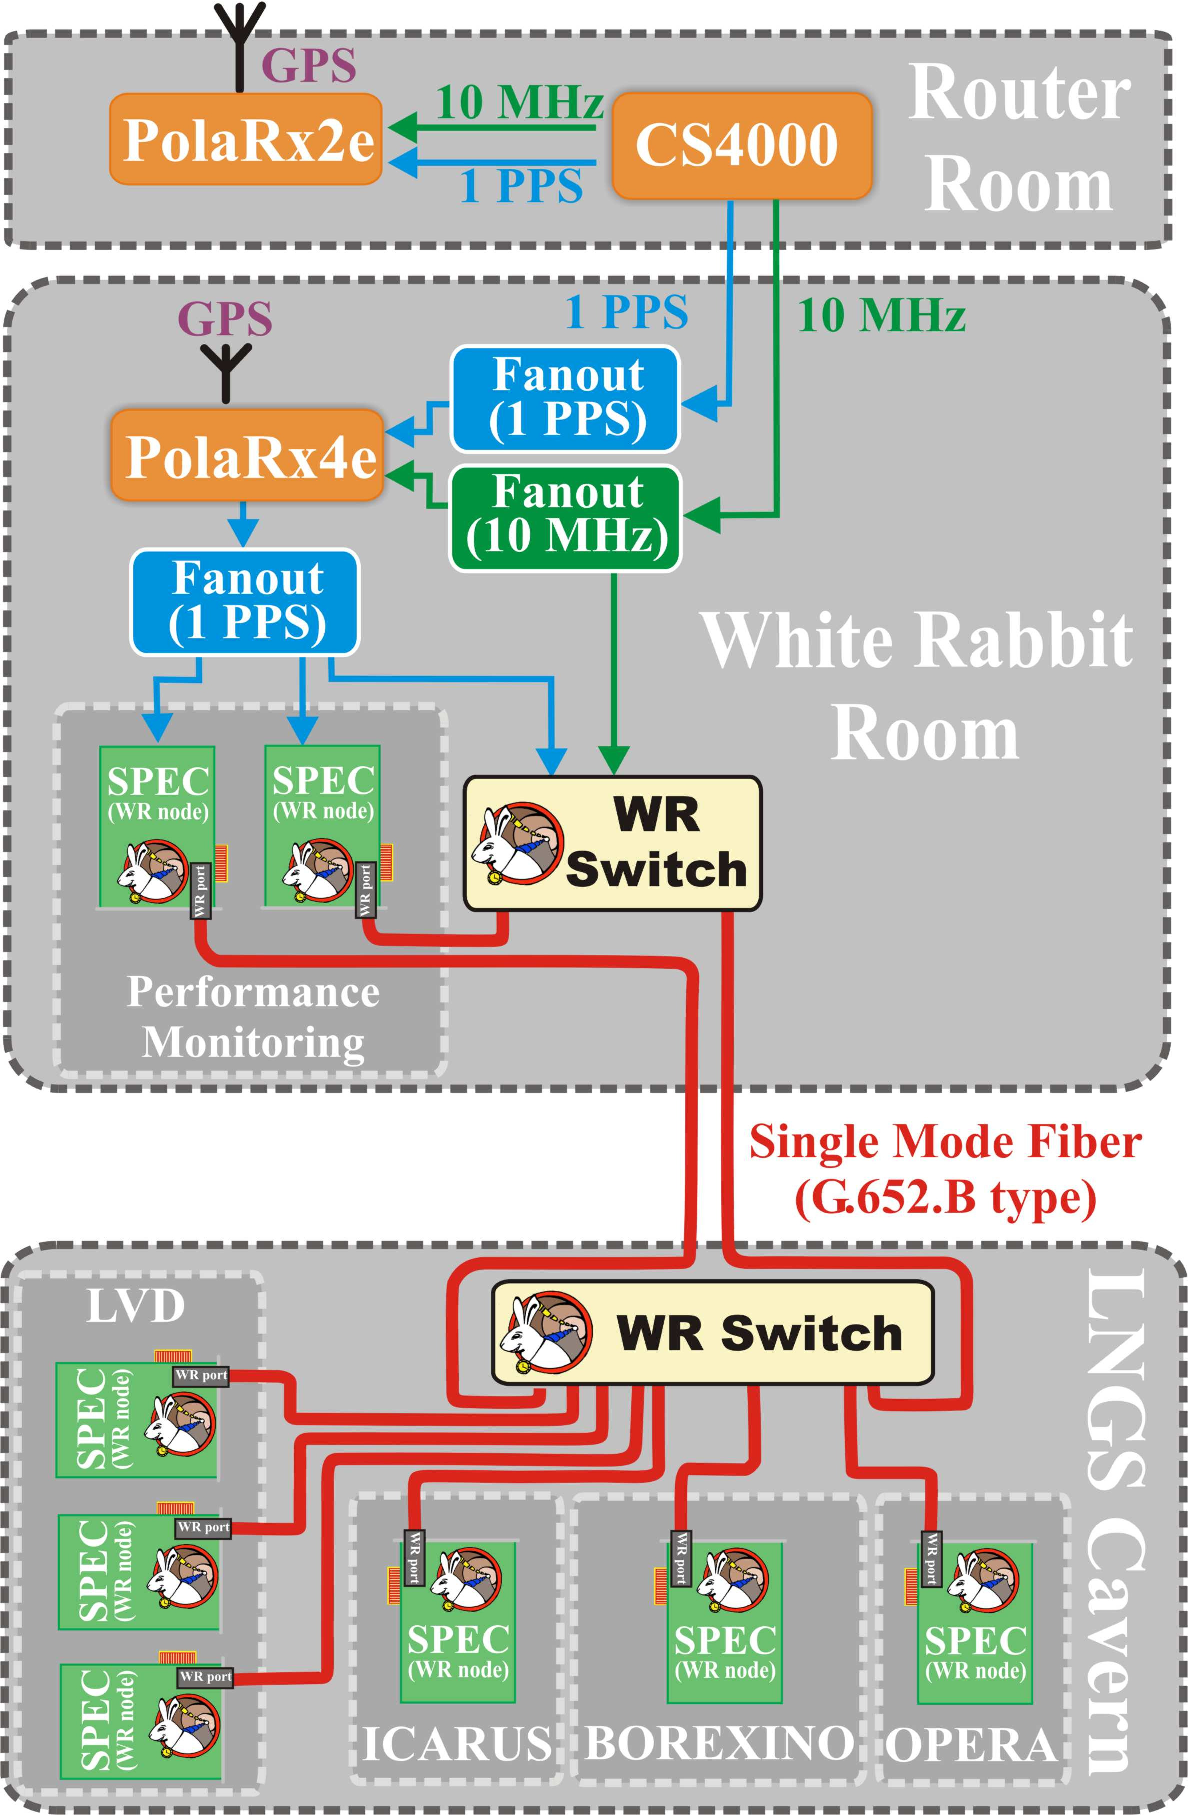
\includegraphics[height=4.0in]{../../figures/applications/CNGS2.eps}
\caption{White Rabbit based synchronization system in Gran Sasso National Laboratory (LNGS).}
\label{fig:wrLNGStiming}
\end{figure}

In the new WR installation (\figurename~\ref{fig:operaTiming} and \figurename~\ref{fig:wrLNGStiming}), 
a common UTC timebase for both remote sites is achieved using two 
identical systems, composed of a Septentrio PolaRx4TR \cite{biblio:PolaRx4e} GPS receiver 
operating in ``common-view" mode and a Symmetricom Cs4000 \cite{biblio:CS4000} Cs atomic clock, 
installed at CERN and LNGS. The Cs atomic clock is a common part of the new and the old 
time transfer systems. 

\figurename~\ref{fig:wrLNGStiming} details the WR setup in LNGS. The Septentrio PolaRx4TR 
accepts the GPS signal and the high stability CS4000 10~MHz signal to generate a timebase whose 
offset with respect to the GPS time can be \modified{derived} 
%known 
a posteriori with very good accuracy. 
The 10~MHz signal of the \modified{Cs atomic} clock (CS4000, installed in the {\it Router Room}) 
is connected (through a fanout) to the 
grandmaster switch. Thus, the timebase of the WR network is that of the  \modified{Cs atomic} clock, 
which in turn, 
can be directly translated to the GPS timebase. The grandmaster in the {\it White Rabbit Room} 
is connected through 8.3~km of fiber to the switch installed in the laboratory cavern. 
This switch serves as a \modified{fanout}
%hub 
for the nodes (SPECs) used in different LNGS experiments (i.e. LVD, 
OPERA, Borexino and ICARUS) as depicted in \figurename~\ref{fig:wrLNGStiming}. 
It is foreseen to extend this very simple network with more switches, possibly 
one for each experiment. 

%\figurename~\ref{fig:wrCERNtiming} presents a very similar WR setup for CERN installation. 

\subsection{Monitoring setup}

The timing performance of the WR installations is carefully monitored.
The PPS output 
of the grandmaster's time source is timestamped by two SPECs 
(\figurename~\ref{fig:wrLNGStiming}). One of the 
SPECs (called \textit{local SPEC}) is connected (through a short fiber) directly to the grandmaster switch (in WR Room), 
thus time-tagging the time source's PPS in 
the time referenced to the grandmaster. The second SPEC (called \textit{loopback SPEC}) 
is connected through 8.3~km of fiber to the 
second switch (located in the cavern), thus time-tagging the time source's PPS in the time 
referenced to the first-layer switch (boundary clock). This SPEC acts as a system loopback which 
provides an estimate of the quality of the time transfer to the SPECs used to time-tag
the input signals in each experiment. The total distance of the loopback is over 16~km 
(\modified{grandmaster $\rightarrow$ boundary clock $\rightarrow$ SPEC}). 


% Additionally, the 10MHz clock outputs of both 
% monitoring SPECs and the cesium clock are analyzed with Agilent E5052B signal source analyzer to
% measure the phase noise, L(f), and estimate the rms jitter.

% In order to compare and monitor differences between the new and the old systems, a PPS signal 
% generated by the old system is time-tagged (SPEC (2) in \figurename~\ref{fig:operaTiming}).

The temperature in the WR Room (in which the SPECs and the grandmaster switch are installed) as well
as the temperatures of the SPECs and Fine Delay modules are monitored. 

% The WR installation at CERN features additionally a roll of 
% fiber exposed to varying external condition (i.e. temperature)\footnote{Data from this setup not available at the time of writing.}. The variation of temperature 
% is logged. The SPEC node, connected to this fiber roll, time-stamps the PPS output of the 
% cesium clock while the 10MHz output of the SPEC is also analyzed with the Agilent device. 


\subsection{Temperature test setup}
\label{sec:tempTestSetup}

%Additionally to 
\modified{Aside from} monitoring the performance and parameters of the deployed system, 
a similar setup was tested in a CTS Climatic Chamber (Type T-40/500) to determine influence 
of the temperature variation on the %system's 
\modified{synchronization} performance. In this setup, a switch acting as a 
free running grandmaster was connected through 11~km of fiber to another switch acting as 
a boundary clock. One SPEC (called \textit{local}) was connected through 10~m of fiber to 
the grandmaster switch. Another SPEC (called \textit{loopback}) was connected to the boundary clock 
switch through 5~km of fiber. \modified{The boundary clock was connected to the grandmaster switch through 11~km 
of fiber.} The skews between the clock of the grandmaster switch and that of 
the boundary clock switch, the \textit{local} SPEC and the \textit{loopback} SPEC were measured using 
LeCroy WavePro 7300A oscilloscope. Monitoring the skew of the recovered clocks
(unlike \mbox{timestamping} the PPS reference) allows to evaluate the performance of the WR-timebase without
additional jitter or inaccuracy introduced by a system using the WR-timebase 
(i.e. TDC on the Fine Delay). 

Different elements of the described setup were placed in the climatic chamber while the rest 
of the setup was placed in a reasonably stable conditions of the laboratory (ambient temperature 
of 26$\pm$1.5 degrees Celsius). 

A temperature cycle consisted of ramping the temperature from 20 to 50 degrees, stabilizing 
at 50 degrees, ramping down to 0 degrees, stabilizing at 0 degrees and ramping up back to 20 degrees. 


% \begin{figure}[!t]
% \centering
% \includegraphics[height=2.0in]{fig/wrCERNtiming.ps}
% \caption{TODO}
% \label{fig:wrCERNtiming}
% \end{figure}


